\FloatBarrier
\section{Annual AC verification on the existing grid}\label{sec:annualac}

Do plans that meet DC flow limits also satisfy AC voltage and thermal limits throughout the year? We test each plan's 8,760-hour dispatch on the existing EPE grid (Table~\ref{tab:ac_scope}). Phase~5 maps portfolio dispatch to buses and tests moving the 2050 batteries to load. Phase~6 compares original sites (reference) with jointly optimised sites and dispatch (joint siting) at the same statewide capacities. In 2050 the reference dispatch leaves 690~GWh unserved and joint siting serves all load, so power delivered also changes.

\begin{table}[!htbp]\centering
\caption{Scope of the DC and AC checks on the existing grid.}\label{tab:ac_scope}
\small
\begin{tabular}{@{}l >{\raggedright\arraybackslash}p{0.36\linewidth} >{\raggedright\arraybackslash}p{0.44\linewidth}@{}}
\toprule
Power flow & Intact network (N-0) & Single outage (N-1) \\
\midrule
DC & Branch MW, normal ratings & Branch MW, emergency ratings \\
AC & Normal bus voltage, 7 cases (Phases~5 and~6) & Emergency voltage and branch MVA, 4 cases (Phase~6) \\
\bottomrule
\end{tabular}
\end{table}

\paragraph{Intact-grid voltage.} We solve all 1,489 buses and screen the 150 physical MG buses at 230~kV and above. A new violation crosses a bus-specific normal limit by more than 0.0001~p.u.\ in a direction clear in the intact snapshot. As in Phase~5, PQ buses retain snapshot reactive injections, regulated buses hold voltage without reactive limits, and the slack bus balances losses.

\begin{figure}[!htbp]\centering
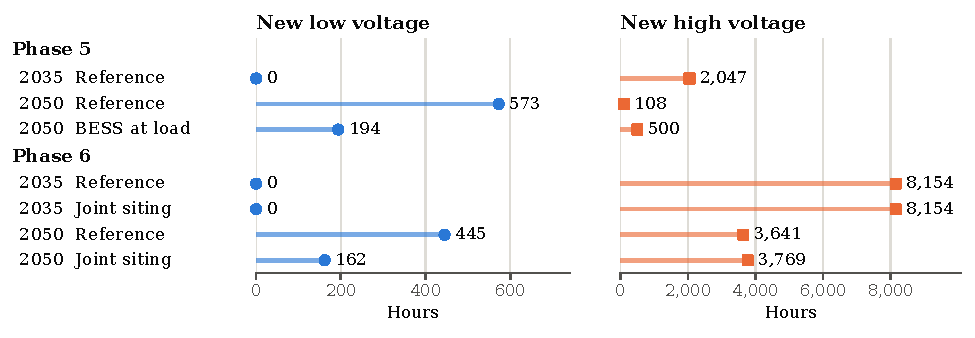
\includegraphics[width=0.96\linewidth]{figures/annual_ac_n0.pdf}
\caption{Hours with new low or high voltage during intact operation, out of 8,760 per case. The two directions can occur in the same hour. Each panel has its own horizontal scale.}\label{fig:annual_ac_n0}
\end{figure}

Both 2035 Phase~6 plans have 8,154 new high-voltage hours. In 2050 both siting experiments trade fewer low-voltage hours for more high-voltage hours (Figure~\ref{fig:annual_ac_n0}). In Phase~6, hours with either violation fall from 3,998 to 3,931. Independent MATPOWER solves \citep{zimmerman2011matpower} reproduce every hourly voltage flag in all 61,320 cases, with a maximum voltage magnitude difference of $1.97\times10^{-9}$~p.u.

\FloatBarrier
\subsection*{Single outages in Phase 6}
Each plan faces the same 437 non-islanding outages as in the DC study every hour (242 lines and 195 transformer branches). The 44 islanding candidates remain outside the screen. For 69 outages, dedicated end reactors leave service with their branch. Independent bus shunts stay in service. Scheduled injections are held through each outage, subject to the same slack and voltage controls as in intact operation.

\paragraph{What counts as new?} Among the 555 monitored branches, we screen those still in service after each outage. For each, we compare the larger of its two terminal MVA flows, $\max(|S_{\rm from}|,|S_{\rm to}|)$, with the emergency rating (0.001~MVA tolerance). An overload is new if that branch was within its rating under the same outage applied to the original network snapshot. For voltage we compare each monitored bus with the \emph{same plan and hour} before the outage, using that bus's emergency limits and the same 0.0001~p.u.\ tolerance in both states. This counts a bus that crosses a limit and excludes a pre-existing violation that deepens.

\begin{figure}[!htbp]\centering
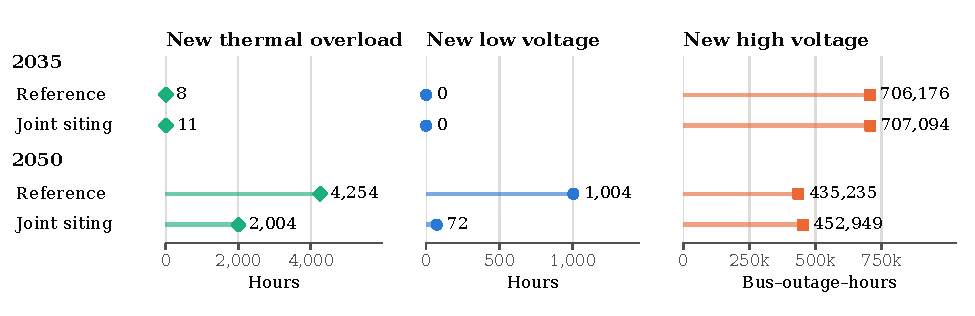
\includegraphics[width=0.98\linewidth]{figures/annual_ac_n1.pdf}
\caption{Phase~6 single-outage checks. The first two panels count distinct hours with at least one new violation. The third counts each affected bus for each outage and hour. All four plans have at least one outage that introduces high voltage in every hour.}\label{fig:annual_ac_n1}
\end{figure}

\begin{table}[!htbp]\centering\small
\caption{Severity and coverage of Phase~6 single-outage results. A thermal event is one branch--outage--hour and a low-voltage event is one bus--outage--hour. Peak loading is for newly overloaded combinations only. Minimum voltage covers all monitored buses in solved cases. Unsolved cases are excluded from violation counts and extrema.}\label{tab:annual_ac_n1}
\begin{tabular}{@{}llrrrrr@{}}
\toprule
Year & Siting & \shortstack[r]{New thermal\\events} & \shortstack[r]{New low-voltage\\events} & \shortstack[r]{Peak loading\\(\% of rating)} & \shortstack[r]{Min.\ voltage\\(p.u.)} & \shortstack[r]{Unsolved\\cases} \\
\midrule
% Use expandable input between booktabs rules.
\csname @@input\endcsname tables/annual_ac_n1_rows.tex
\bottomrule
\end{tabular}
\end{table}

\paragraph{Thermal loading and voltage.} The annual DC check finds zero new overloads in all four plans. AC gives a different assessment because losses and voltage affect active flows, and reactive power contributes to equipment loading. In 2035 the newly overloaded combinations peak at 101.51\% of rating, and neither plan introduces low voltage under an outage. In 2050 joint siting cuts new thermal events by 93\% and reduces hours with new low voltage from 1,004 to 72. High-voltage exposure moves in the opposite direction, rising from 435,235 to 452,949 bus--outage--hours (Figure~\ref{fig:annual_ac_n1}). These counts describe the reach of the enumerated outages. Estimating their likelihood would require outage probabilities.

\paragraph{Which minimum voltage?} Of 15,312,480 outage cases, 15,312,439 converged. For seven 2050 reference cases, direct AC solves reached two different steady-state solutions. Starting from the same hour's intact solution, we gradually removed the affected equipment at fixed scheduled injections. MATPOWER reproduced the same solution at two step sizes in all seven cases. With this rule the 2050 reference annual minimum is \textbf{0.6952~p.u.}, compared with 0.8715~p.u.\ under joint siting (Table~\ref{tab:annual_ac_n1}). As a sensitivity, direct MATPOWER solves give a reference annual minimum of 0.5145~p.u.\ in a different hour. With the selected solutions, MATPOWER reproduces all hourly counts and extrema to the reporting tolerances. The remaining 37 reference and four joint-siting cases in 2050 have undetermined outcomes.
\FloatBarrier
